\chapter{Trabalho desenvolvido}
\label{cha:trabalho desenvolvido}

A solução proposta para a resolução do problema apresentado no capítulo \ref{cha:introdução} é um sistema separado em três fases, cada uma delas ligada a um elemento físico: o Arduino, o telemóvel e a base de dados (alocada num computador). 
Na figura \ref{fig:arquitetura} é possível ver um esquema da arquitetura do sistema desenvolvido.
Assim as seguintes secções são referentes às três fases do sistema.

\begin{figure}[hbtp]
	\centering
	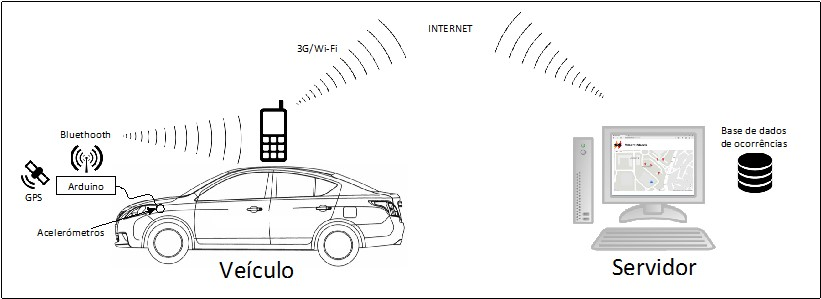
\includegraphics[width=14cm]{arquitetura}
	\caption{Arquitetura do sistema}
	\label{fig:arquitetura}
\end{figure}

\section{Funcionamento do Arduino}
\label{sec:funcionamento_do_arduino}
O código Arduino está dividido em três partes: inicialização, setup e loop, sendo que a inicialização e setup são apenas executadas uma vez enquanto que loop é executada até que o Arduino seja desligado ou alguma parte do código force uma paragem.
No apêndice \ref{cha:codigo_do_arduino} é possível ver o código desenvolvido para o Arduino, o qual é explicado de seguida.

\begin{itemize}
\item Na zona de declarações são incluídas as bibliotecas referentes ao acelerómetro, ao cartão de memória e ao GPS.
São também definidos os modos de escrita no cartão de memória, os portos de ligação de comunicação do GPS e criadas variáveis globais referentes ao GPS e ao acelerómetro.
Além disso, são criadas variáveis globais de controlo do código, variáveis de passagem de parâmetros entre vários ciclos da função \emph{loop} e declaração de constantes que serão utilizadas diversas vezes ao longo do código, facilitando a alteração do seu valor em todo o código, caso tal se mostre necessário.

\item Na função \emph{setup} são declaradas as frequências de comunicação entre o Arduino e o telemóvel e entre o GPS e o Arduino.
São também inicializados dois \emph{leds} como elementos de saída de informação e um botão como entrada de informação ao qual foi atribuído o estado de “desligado” a ambos os \emph{leds}.
Por fim, são executadas as funções de inicialização do leitor do cartão de memória e do acelerómetro, SD\textunderscore init e AccelInit respectivamente, ambas explicadas mais á frente.

\begin{figure}[hbtp]
	\centering
	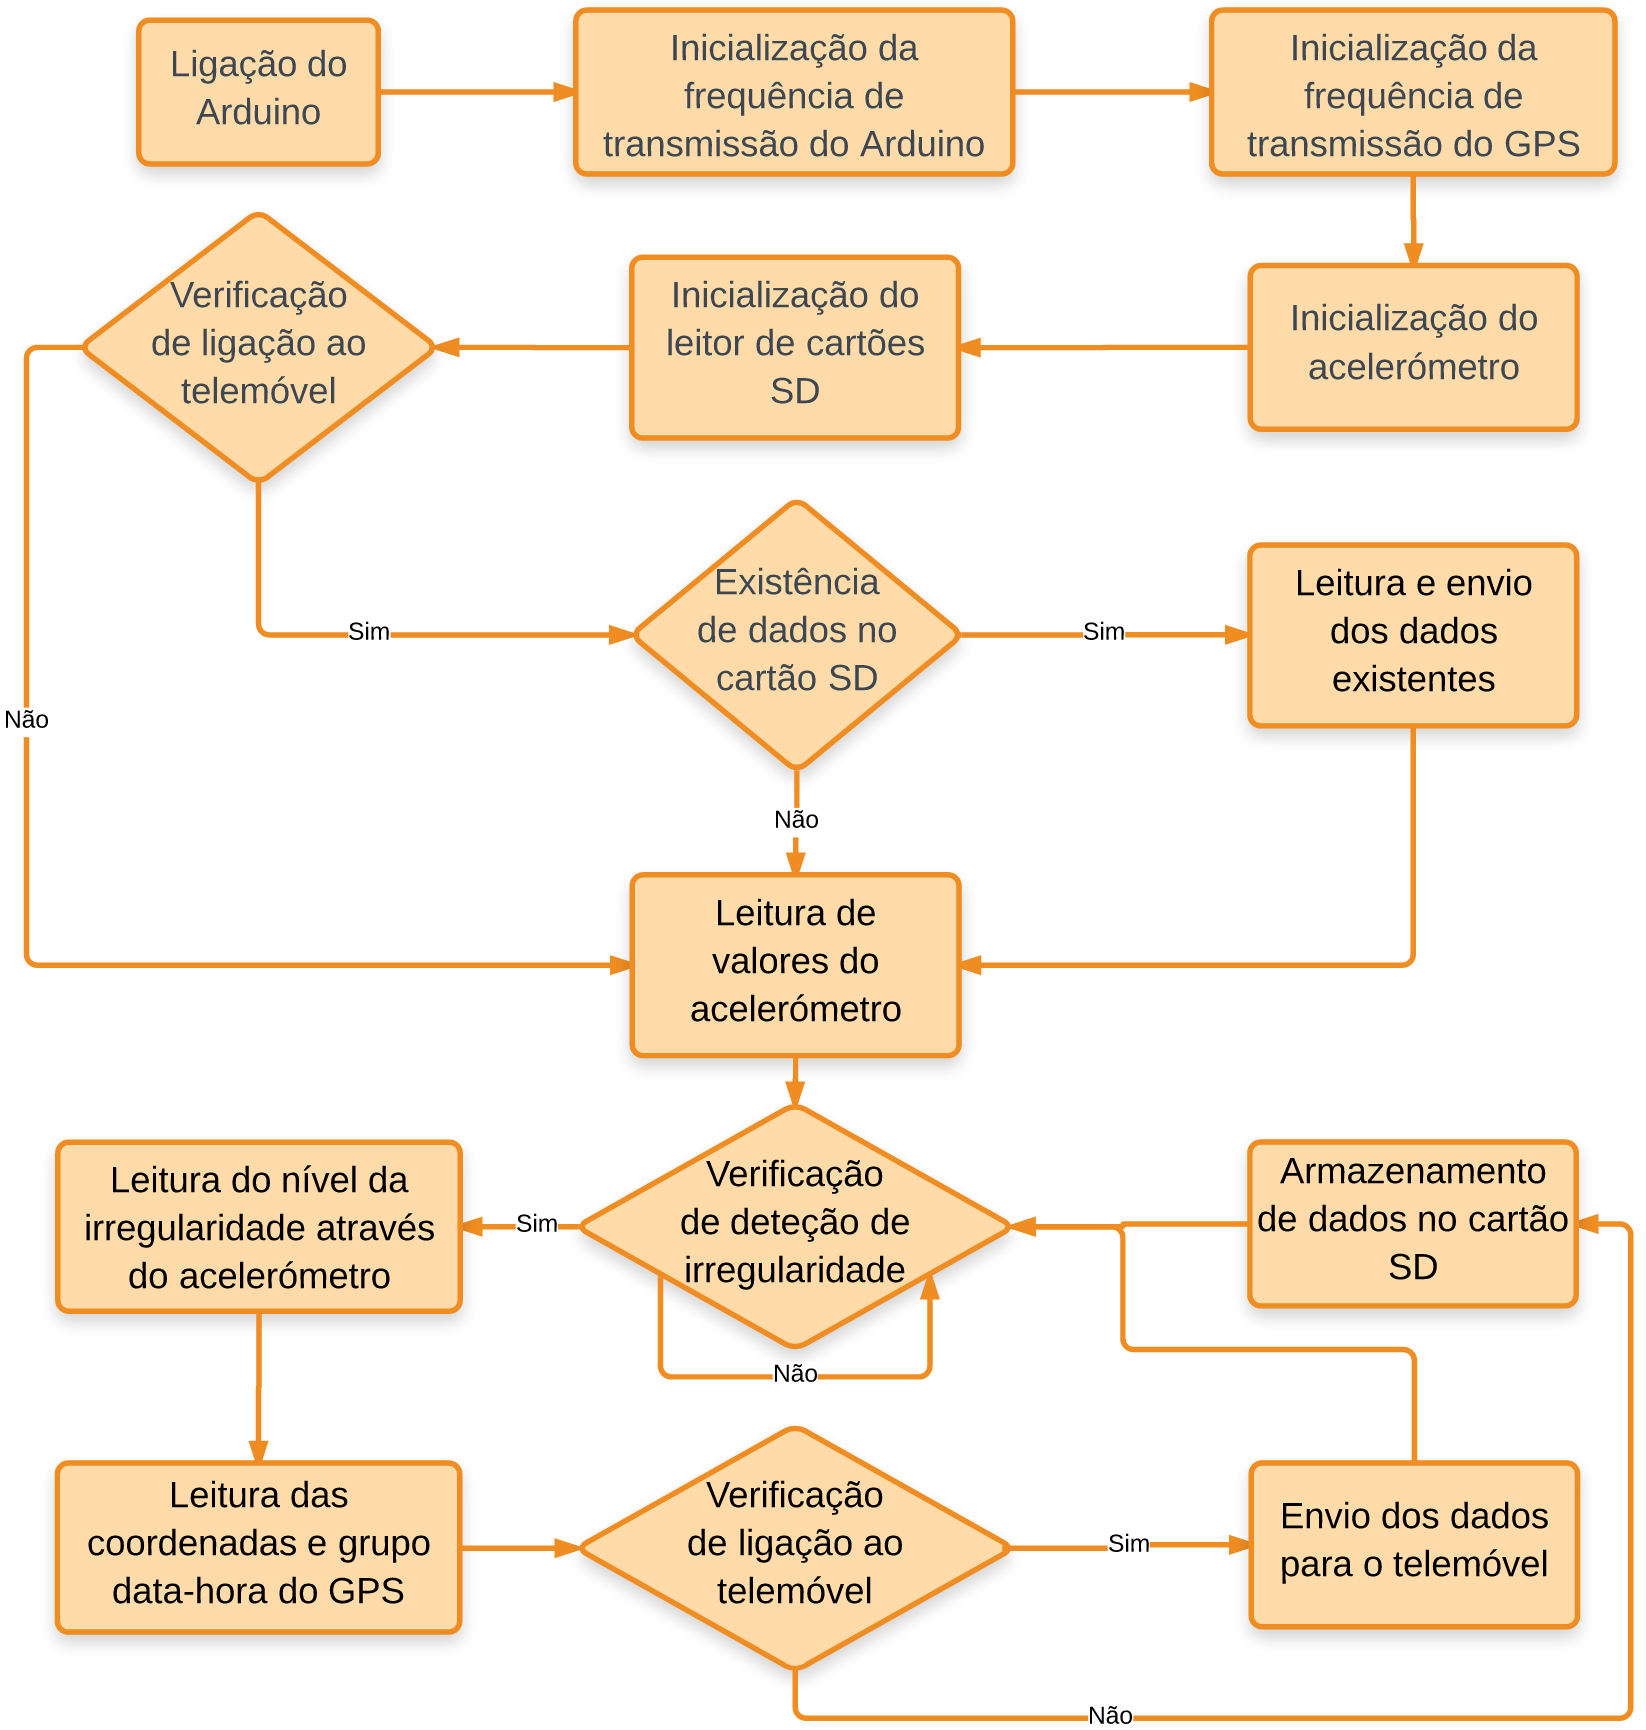
\includegraphics[height=10cm]{FlowArduino}
	\caption{Fluxograma referente ao código Arduino}
	\label{fig:Fluxograma_referente_ao_código_arduino}
\end{figure}

\item A função \emph{loop}, embora executada de uma forma constante, contém um código bastante simples mas importante.
A função começa por verificar se existe informação disponível para leitura no módulo Bluetooth, relativa à ligação.
Caso tal se verifique, essa informação é lida e comparada com a leitura anterior, para que seja possível determinar se a ligação ao módulo Bluetooth do Arduino sofreu alguma alteração, nomeadamente, quanto à ligação com a aplicação desenvolvida para esta dissertação.
Na hipótese desta alteração se verificar, é avaliada se a ligação foi estabelecida ou cortada entre o Arduino e o telemóvel, sendo que, no caso de ser estabelecida, é executada a função ReadSD para leitura do cartão de memória e um \emph{led} de controlo é aceso.
Caso contrário, o mesmo \emph{led} de controlo é desligado. 
De seguida são lidos os valores de aceleração dos eixos X, Y e Z, provenientes do acelerómetro, armazenados e comparados com a leitura anterior para verificação da existência de alguma irregularidade no asfalto.
A maneira como esta comparação é realizada será explicada mais à frente.
Caso seja detectada alguma irregularidade, um dos \emph{leds} de controlo pisca e são armazenados, numa variável \textbf{S}, os valores do nível da irregularidade, bem como o grupo data-hora proveniente do GPS.
Seguidamente é verificada a ligação entre o Arduino e a aplicação e caso esta exista, os valores de \textbf{S} são enviados directamente para o telemóvel.
Se a ligação não existir, os valores de \textbf{S} são transferidos para o cartão de memória para que possam ser transmitidos para o telemóvel assim que exista uma ligação estável com o mesmo.
Por fim, os valores actuais do acelerómetro são armazenados para que possam ser comparados na próxima execução da função \emph{loop}.
\end{itemize}

\section{Funções adicionais}
\label{sec:funcoes_adicionais}

\subsection{SD\textunderscore init}
\label{sub:sd_init}

Esta função serve para inicializar o leitor de cartões SD.
Nesta é chamada a função \emph{begin} da biblioteca \emph{SD} e verificada a resposta dessa mesma função.
Caso a resposta seja o valor 10, um \emph{led} de controlo pisca para que o utilizador saiba que a inicialização ocorreu com sucesso e é verificada a existência de um ficheiro com informação previamente armazenada sobre irregularidades detetadas anteriormente.
Caso exista esse ficheiro, este é aberto de modo a que se possam juntar novos valores de irregularidades detetadas, caso contrário, o ficheiro é criado para futuros armazenamentos.

\subsection{WriteSD}
\label{sub:writesd}

Para que o cartão de memória possa armazenar dados é apenas necessário abrir um ficheiro em modo escrita.
A função \emph{open} da biblioteca do SD está desenhada de forma a que, quando é pedido para abrir um ficheiro, este seja procurado no cartão de memória e caso não exista nenhum ficheiro com esse nome, então é criado um novo ficheiro vazio, com o nome inserido e posteriormente aberto.
Para que possa ser mais fácil ao utilizador saber se a abertura e escrita do ficheiro foi feita com sucesso, um \emph{led} pisca duas vezes.
No final resta apenas fechar o ficheiro para que tudo fique guardado devidamente.

\subsection{ReadSD}
\label{sub:readsd}

Semelhante à função de escrita, a função de leitura tenta abrir um ficheiro com o nome pretendido, embora neste caso, se o ficheiro desejado não existir, não é criado um novo pois se este não existir significa que não existem dados pendentes para envio.
Quando um ficheiro é lido com sucesso, os seus valores são enviados pela porta série do Arduino para o telemóvel, o ficheiro é fechado e eliminado, de modo a que não sejam enviados dados duplicados.
O código está protegido de modo a que os dados sejam apenas enviados para um telemóvel com a aplicação desenvolvida pois previamente foi recebida uma mensagem de controlo enviada pela própria aplicação, informando o estado da ligação, evitando que os dados sejam enviados para ligações desconhecidas.

\subsection{AccelInit}
\label{sub:accelInit}

Nesta função o acelerómetro é ligado e são determinados os valores de sensibilidade do mesmo.
É também feita a inicialização de valores para queda livre e batida que não são utilizados na dissertação.
Esta funcionalidade foi mantida para possíveis aplicações futuras e uma deteção mais pormenorizada das irregularidades.
Seguidamente, um \emph{led} de controlo pisca para o utilizador saber que a inicialização foi bem sucedida.

\subsection{Accel}
\label{sub:accel}

Na função \emph{Accel} é realizado o processamento dos valores de aceleração dos três eixos do acelerómetro para determinar a classificação da irregularidade detetada.
Embora o processo seja simples, é eficaz e semelhante ao método \textbf{Z-DIFF} apresentado em \cite{Mednis2011}, mas aplicado aos três eixos de aceleração em simultâneo.
O método baseia-se em detetar a existência de desvios superiores a um limite previamente determinado, tendo sido considerados valores múltiplos de 100 nesta dissertação.
Assim, é feita uma subtração de valores sucessivos de aceleração dos eixos e avaliado o valor absoluto dessa diferença.
O valor atribuído à irregularidade é o mais baixo dos três desvios.
Na figura \ref{fig:grafico_de_uma_irregularidade_detetada} é possível ver o gráfico de uma deteção, em que o nível atribuído foi 4.

\begin{figure}[hbtp]
	\centering
	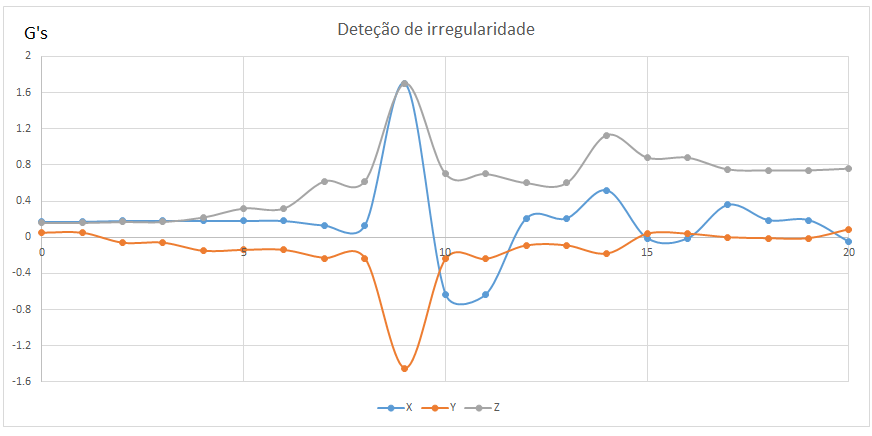
\includegraphics[width=14cm]{irregularidade}
	\caption{Gráfico de uma irregularidade detetada}
	\label{fig:grafico_de_uma_irregularidade_detetada}
\end{figure}

\subsection{displayGPS}
\label{sub:displayGPS}

A função \emph{displayGPS} é sem dúvida a mais elaborada nesta secção do trabalho devido aos dados enviados pelo GPS, muito extensos e, neste caso, não necessários, além de se encontrarem num formado não muito fácil de separar.
A função é chamada dentro da função \emph{loop} de modo a registar tanto o conjunto data-hora como as coordenadas em que a irregularidade foi detetada.
Quando é chamada, faz uma leitura dos valores que o sensor GPS recebe dos satélites e percorre-os até encontrar o texto ``GPRMC'', a partir do qual vem toda a informação necessária e armazena todos esses valores num vetor de strings (sequências de caracteres).
O passo seguinte consiste em percorrer o vetor e retirar apenas os segmentos relevantes, pela ordem desejada, neste caso, começando pela latitude e longitude, seguindo-se a data e por fim a hora.
Quando estes quatro parâmetros são armazenados, a função muda o valor de uma variável de controlo e o código prossegue.

\subsection{FTOA - Float to ASCII}
\label{sub:FTOA}

Dada a forma em que os valores das coordenadas do GPS são recebidos, é necessária fazer uma conversão para um formato mais simples de transmitir e como o processo de conversão é executado diversas vezes, foi criada uma função que evita repetição do código.
Os dados enviados pelo GPS, relativos às coordenadas vêm no formato DDS – Degree Decimal Minutes (Graus e Minutos Decimais em Português) e apresentam o formato (1) da figura \ref{fig:formatos_de_apresentacao_de_coordenadas}.
Tal como se pode verificar, existem seis parâmetros neste formato, nomeadamente graus, minutos  e hemisfério, três para a latitude e outros três para a longitude. 
Um formato mais simples é o DD – Decimal Degree (Graus Decimais em Português), também apresentado na figura \ref{fig:formatos_de_apresentacao_de_coordenadas}, no ponto (2).
Neste formato existem apenas quatro parâmetros (graus e hemisfério) que podem ser reduzidos a dois, se forem considerados graus negativos, representando o hemisfério a que a latitude ou longitude se referem, sendo assim necessário enviar menos dados para representar a mesma quantidade de informação, tornando o processo mais rápido.
A conversão de DDS para DD é simples, sendo apenas necessário dividir a parte dos minutos decimais por 60 (convertendo minutos para graus) e somar esse valor aos graus já existentes.
Como os valores que são recebidos do GPS vêm em \emph{strings}, é necessário convertê-los para formato numérico, através da função atoi (ASCII to Integer, ASCCI para inteiro em português) que já existe nas bibliotecas do Arduino e posteriormente voltar a converter para formato de \emph{string}.
Apesar de ser possível escrever um valor numérico numa string, quando esta operação é feita, apenas duas casas decimais são utilizadas e para que as coordenadas possam apresentar um elevado grau de precisão são necessárias quatro casas decimais, sendo assim necessária a criação desta nova função de modo a reter tantas casas decimais quanto as desejadas.

\begin{figure}[!htbp]
	\centering
	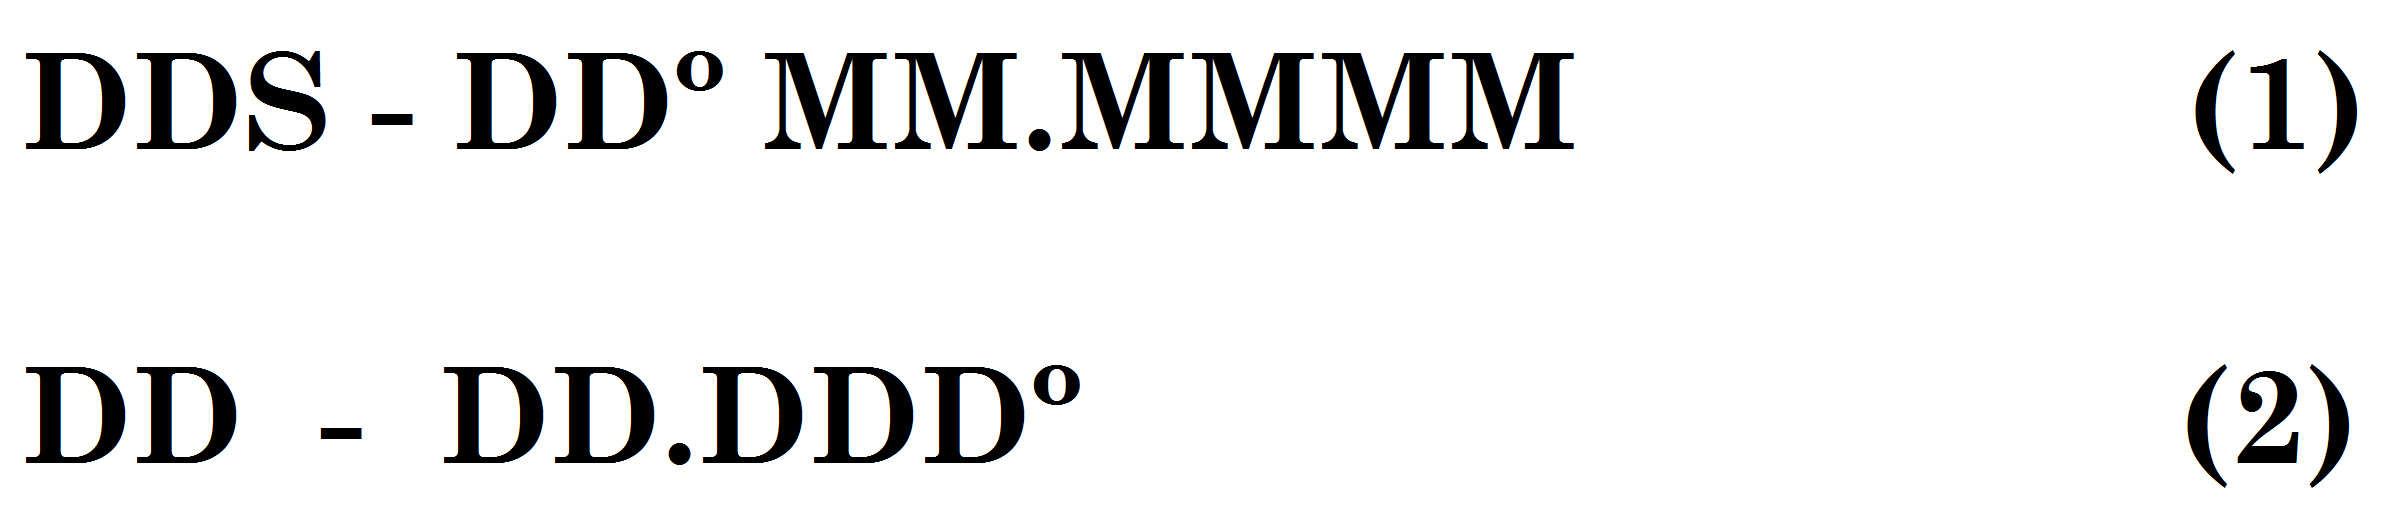
\includegraphics[height=2cm]{Coordenadas}
	\caption{Formatos de apresentação de coordenadas}
	\label{fig:formatos_de_apresentacao_de_coordenadas}
\end{figure}

\section{Funcionamento do Android}
\label{sec:funcionamento_do_android}

Tal como explicado na secção \ref{sec:android}, o método escolhido para a programação Android foi a MIT App Inventor 2, no website http://ai2.appinventor.mit.edu.
Por correr num web browser, todo o processamento e compilação de código é feito no servidor e não no computador local, tornando o processo de criação mais rápido.
Além disso, a sua programação por blocos torna o processo muito mais compreensível uma vez que os blocos existentes mostram quais as funcionalidades de cada tipo de dados, desde números a vetores.
Este modo de programação mostrou-se muito prático dada a inexperiência de desenvolvimento de aplicações para telemóvel.
A existência de apenas quatro botões torna esta aplicação bastante fácil de utilizar, pois cada botão tem a sua função devidamente identificada, tal como é possível ver na figura \ref{fig:Aspeto_da_aplicação_Smart_Shock}.


\begin{figure}[!htbp]
	\centering
	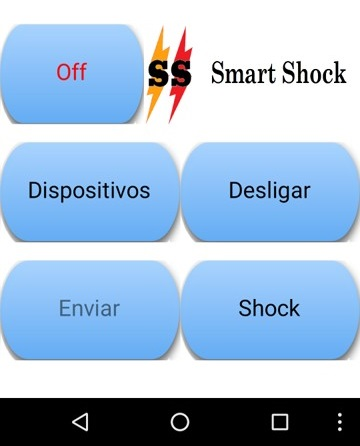
\includegraphics[width=5cm]{AppVisual}
	\caption{Aspeto da aplicação Smart Shock}
	\label{fig:Aspeto_da_aplicação_Smart_Shock}
\end{figure}

A base do código da aplicação é um ciclo \emph{while} que corre desde que a aplicação seja executada, semelhante à função \emph{loop} do Arduino.
Dentro deste ciclo existem duas condições: uma que verifica se o GPS do telemóvel está a detetar coordenadas e outra que verifica a ligação ao módulo \emph{Bluetooth} do Arduino, bem como um procedimento que verifica a existência de dados armazenados no telemóvel para futuro envio para a base de dados.
O GPS existente no telemóvel é utilizado para que seja possível reportar irregularidades existentes no asfalto mesmo que não se esteja a conduzir, possibilitando todos os transeunte adicionar informações sobre o local em que se encontram.
Sempre que são detetadas coordenadas disponíveis, um botão com o texto \emph{``Shock''} fica ativo e sempre que é pressionado são armazenadas as coordenadas atuais, bem como a data e hora presentes para um posterior envio para a base de dados.
Para que estas ocorrências possam ser diferenciadas das detetadas pelo acelerómetro montado no Arduino, o código que lhe é atribuído tem um valor único, facilitando assim a diferenciação entre os dois tipos de irregularidades.

No que toca à ligação a um módulo \emph{Bluetooth}, sempre que esta existe, é enviado um código para o dispositivo ao qual foi feita a ligação.
Este código serve para o Arduino saber que o dispositivo que se encontra ligado tem a aplicação a correr, evitando assim que os dados recolhidos por este sejam enviados para um dispositivo desconhecido.
Depois de ser feita a ligação, o código fica a ``escutar'' o Arduino até que o mesmo envie alguma informação para o telemóvel e quando tal acontece, os vários conjuntos de dados recebidos são escritos e organizados numa lista temporária.
Após a divisão ser feita, a lista é percorrida e os dados são enviados para o cartão de memória do telemóvel ou para a base de dados, dependendo da existência de ligação Wi-Fi.
Esta ligação é verificada a partir de um erro produzido automaticamente pelo sistema Android, sendo emitida uma mensagem de erro com um código específico.
O envio de dados para a base de dados é feito através do método \emph{POST}, tornando possível ocultar os dados enviados, sendo esta uma vantagem no caso de no futuro serem desenvolvidas contas de utilizador em que certas informações devem permanecer confidenciais.
Se a ligação à Internet não existir, os dados são armazenados no telemóvel para um futuro envio, sendo necessário pressionar um botão existente na aplicação.
Este botão serve também para informar o utilizador que tem dados armazenados no dispositivo, uma vez que o botão nem sempre se encontra ativo.

Quanto à seleção de dispositivos \emph{Bluetooth}, é mostrada uma lista dos dispositivos com que o telemóvel está emparelhado.
No caso de ser a primeira vez que um determinado telemóvel se liga ao Arduino, é necessário fazer o emparelhamento fora da aplicação, como para qualquer outro dispositivo.
Quando a aplicação é terminada, é enviada uma mensagem para o Arduino de modo a que este saiba que não é possível enviar mais informação sobre irregularidades e armazene todas as deteções nesse cartão de memória.
Na figura \ref{fig:Fluxograma_referente_ao_código_android} é possível compreender qual o ciclo de funcionamento da aplicação, sendo que no lado esquerdo se encontra o ramo principal e o ciclo que está sempre em funcionamento enquanto a aplicação estiver aberta.
Já do lado direito é possível ver quais os procedimentos realizados quando os botões ``Shock'' e ``Enviar'' são pressionados.

\begin{figure}[hbtp]
	\centering
	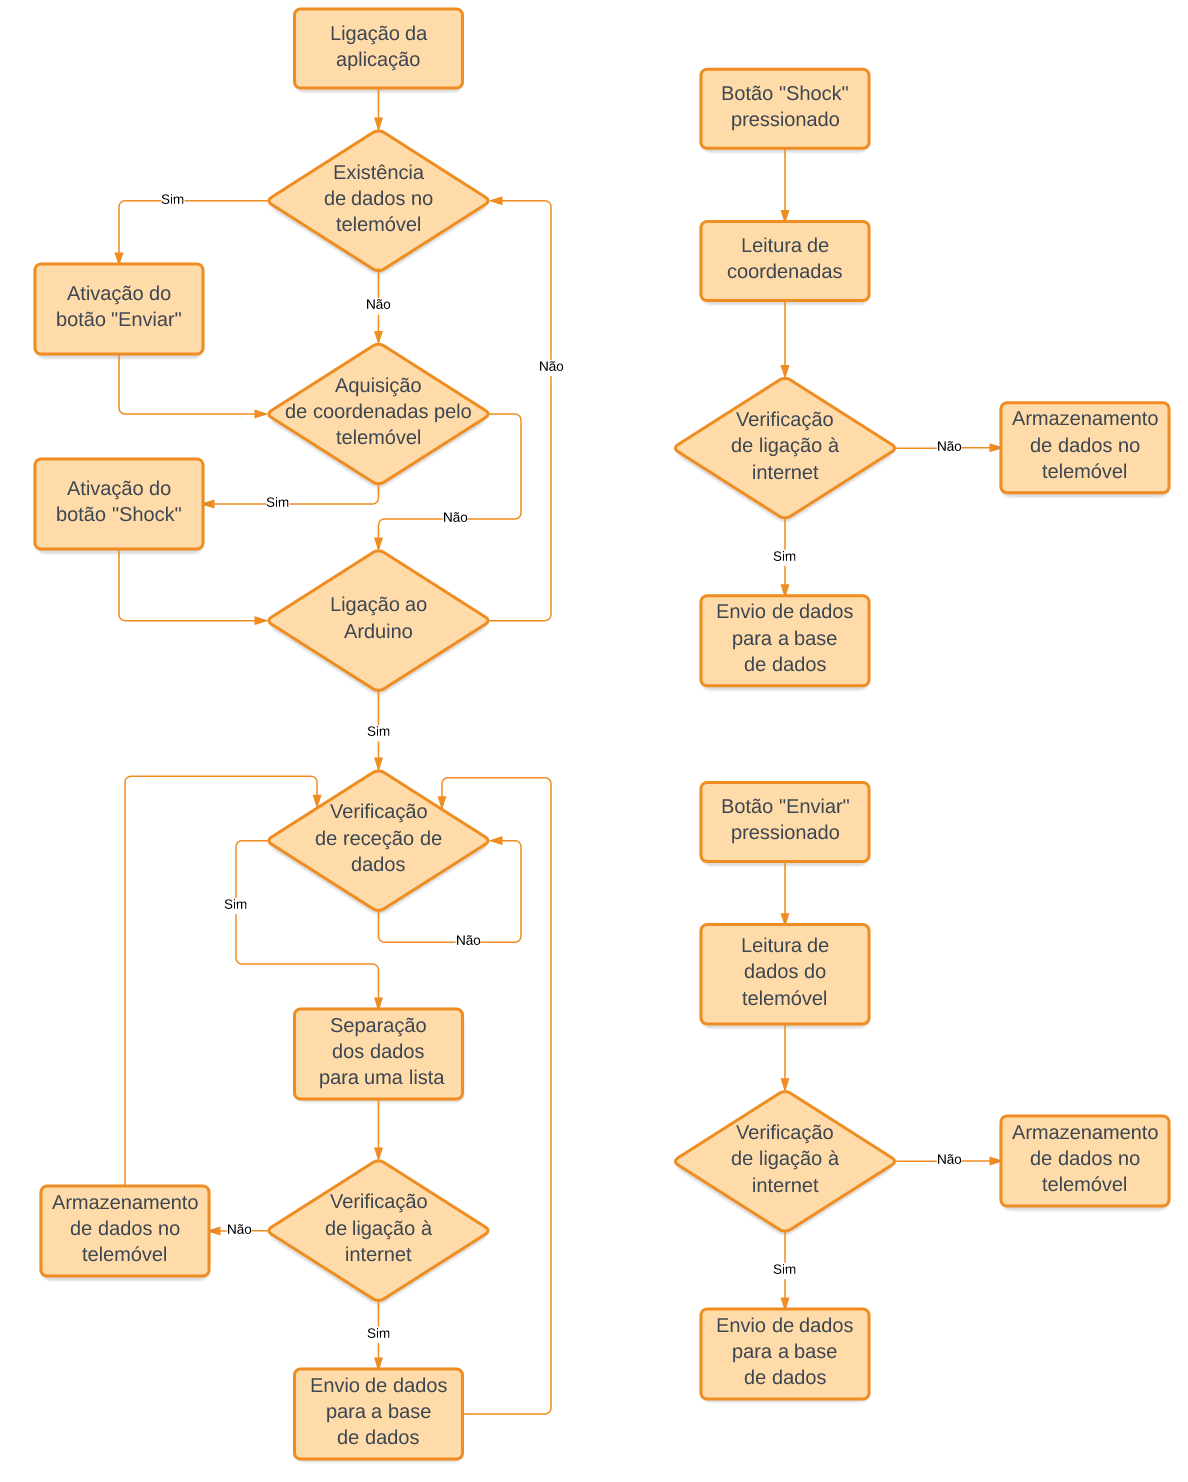
\includegraphics[height=19cm]{FlowAndroid}
	\caption{Fluxograma referente ao código Android}
	\label{fig:Fluxograma_referente_ao_código_android}
\end{figure}

No apêndice \ref{cha:codigo_da_aplicacao} são apresentados alguns dos blocos construidos para o funcionamento da aplicação para uma melhor compreensão do funcionamento do App Inventor.
\newpage

\section{Base de dados}
\label{sec:Base_de_dados}

De modo a que seja possível consultar as irregularidades, foi necessário desenvolver uma base de dados onde ficassem armazenadas as coordenadas, data, hora e intensidade da irregularidade detectadas.
Esta base de dados foi desenvolvida em MySQL e contém cinco campos, sendo eles o ID (campo de identificação de cada entrada), a intensidade da irregularidade, a latitude e a longitude da irregularidade e também o conjunto data-hora, utilizando apenas uma variável.
Esta base de dados pode ainda ser consultada e alterada por um administrador da mesma, caso este ache necessário de modo a inserir novas funcionalidades no projeto.

\section{WebSite}
\label{sec:website}

No apêndice \ref{cha:codigo_do_site} é possível ver o código das páginas referidas no texto que se segue.
Através desse texto é possível recriar todo o sistema desenvolvido.

\subsection{home.php}
\label{sub:home.php}

Esta é a página principal da parte \emph{web} desta dissertação.
Nela é possível ver-se o logótipo e o nome utilizados neste projeto e também um mapa que contém todas as irregularidades detetadas ou inseridas manualmente, referindo a intensidade das mesmas.
Para que essas irregularidades possam ser mostradas, é percorrida toda a base de dados através de uma \emph{query} (pesquisa, em português) de MySQL em que são devolvidos os valores de latitude, longitude e intensidade.
Depois, utilizando a API Google Maps, todos os pontos são marcados no mapa, sendo que no seu sinalizador está indicada a intensidade da irregularidade, como se pode ver na figura \ref{fig:home.php}.
No caso de existirem várias irregularidades muito próximas fisicamente, a interface agrupa-as automaticamente, informando quantas se encontram nessa zona.
A cor destes agrupamentos é alterada consoante o número de itens aglomerados, tornando assim mais fácil a deteção de locais com elevado número de ocorrências.

\subsection{store.php}
\label{sub:store.php}

A página store não contém nenhuma componente gráfica para consulta de informação pois destina-se apenas ao armazenamento de dados na base de dados.
Quando o telemóvel envia dados, é este o destino e como tal, tem que existir algum processamento dos dados recebidos.
A informação recebida é exemplificada na figura \ref{fig:informacao_tipo_adicionada_na_base_de_dados} e vem dividida em quatro \emph{strings}: força, latitude, longitude e data-hora, sendo portanto necessário fazer uma conversão para o formato correto e consequente armazenamento em variáveis locais.
De seguida é feita uma \emph{query} MySQL para que seja possível fazer o armazenamento na base de dados, sendo emitida uma mensagem de controlo para o telemóvel de modo a dar informação sobre o sucesso ou falha deste armazenamento.

\begin{figure}[htp]
	\centering
	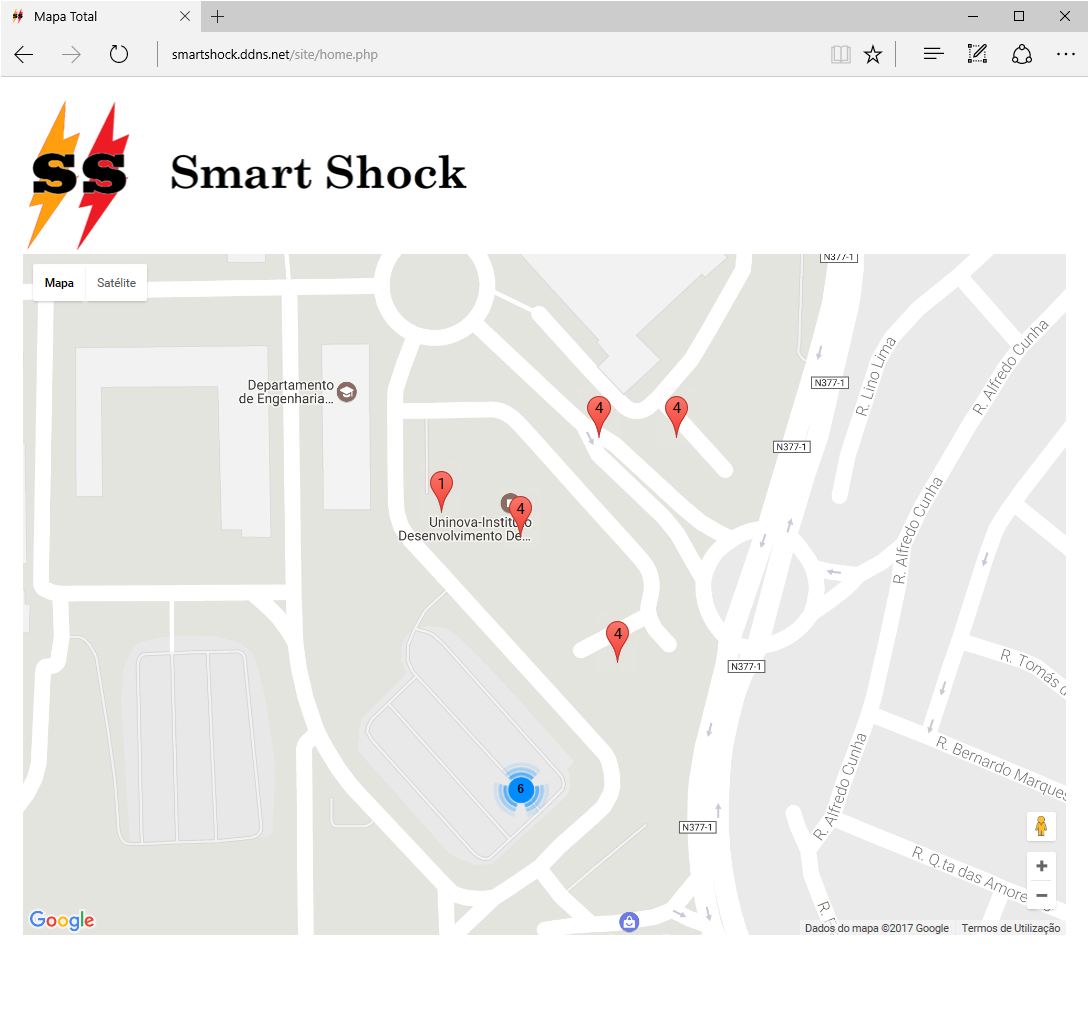
\includegraphics[height=13cm]{home}
	\caption{Página \emph{web home.php}}
	\label{fig:home.php}
\end{figure}

\subsection{listLocations.php}
\label{sub:listlocations.php}

Esta página \emph{web} é bastante semelhante à \emph{home.php}, sendo que aqui apenas é mostrada a localização da irregularidade selecionada na página \emph{listlocations.php} de modo a ser mais fácil descobrir a localização da irregularidade quando esta se encontra agrupada com outras irregularidades existentes nas proximidades, como acontece na figura \ref{fig:home.php}.

\begin{figure}[htbp]
	\centering
	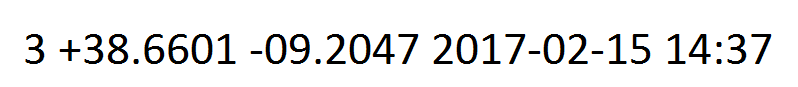
\includegraphics[width=10cm]{dados}
	\caption{Informação tipo adicionada na base de dados}
	\label{fig:informacao_tipo_adicionada_na_base_de_dados}
\end{figure}

\subsection{showLocation.php}
\label{sub:showLocation.php}

Esta página tem a finalidade de consultar todas as irregularidades num formato numérico, ao invés da página \emph{home.php}, em que as irregularidades são apresentadas num mapa.
Tal como apresentado na figura \ref{fig:listlocations.php}, nesta página é possível consultar toda a informação referente a uma irregularidade, incluindo a data e hora em que foi detetada.
Para que seja necessário visualizar a lista de irregularidades, é necessário colocar no endereço o número da página que se deseja visualizar, sendo o valor pré-definido “1”.
Cada uma destas páginas mostra dez entradas da lista de irregularidades e no fundo da página é mostrado um navegador para as diferentes páginas. 
Alinhado com cada irregularidade, existe uma hiperligação para a página \emph{showLocation.php} em que é mostrado no mapa a localização da irregularidade selecionada para uma melhor compreensão dos valores de latitude e longitude.

\begin{figure}[htbp]
	\centering
	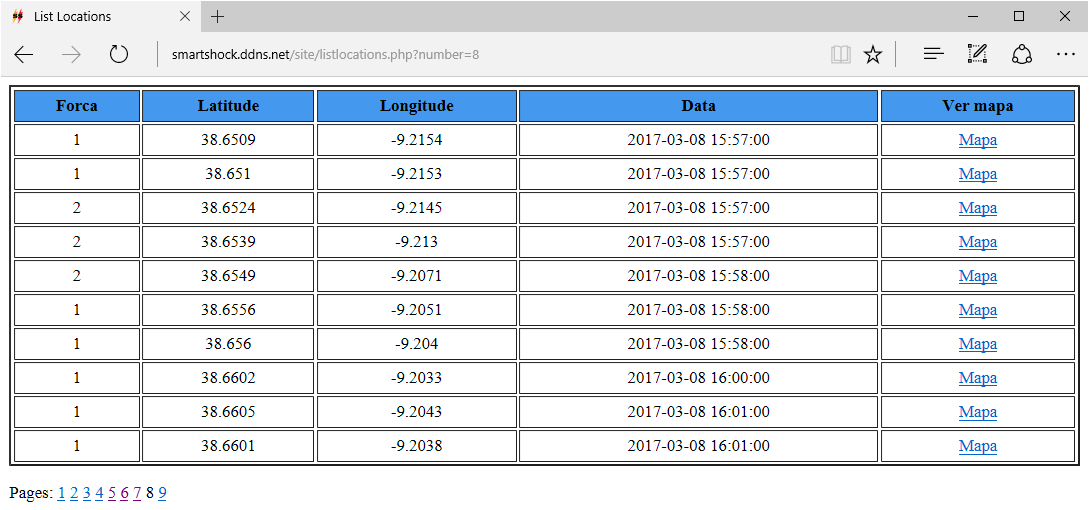
\includegraphics[width=15cm]{listlocations}
	\caption{Página \emph{web listlocations.php}}
	\label{fig:listlocations.php}
\end{figure}

\section{Montagem do sistema}
\label{sec:montagem_do_sistema}

O sistema final foi montado numa PCB desenhada para o Arduino Mega, apesar de ter sido utilizado um Arduino Uno, graças à semelhança dos equipamentos.
A utilização desta PCB deve-se ao tamanho da mesma, sendo assim possível espaçar os componentes mais facilmente, evitando possíveis interferências entre eles e que possibilita uma melhor gestão das ligações.
Foi também necessário utilizar dois reguladores de tensão para converter a tensão de entrada de $12 V$ do automóvel para $5.0 V$ e $3.3 V$.
Apesar do Arduino já conter reguladores semelhantes, existe uma limitação de $200 mA$ na corrente de alimentação, a qual não é suficiente para alimentar o sistema.
São também necessários dois reguladores visto existirem componentes que necessitam de ser alimentados a $5.0 V$ e outros a $3.3 V$ pelo que o regulador LM7805 faz a conversão de $12 V$ para $5.0 V$ e o regulador LM3940 faz a conversão de $5.0 V$ para $3.3 V$.
As figuras \ref{fig:esquematico_do_sistema} e \ref{fig:montagem_real_do_sistema} representam um esquema da montagem e a montagem real do sistema, respetivamente.
A montagem da figura \ref{fig:montagem_real_do_sistema} foi então instalada num veículo de testes para validação dos resultados, abaixo do amortecedor para evitar a deterioração dos dados recolhidos, como mostra a figura \ref{fig:carro}.

\begin{figure}[htbp]
	\centering
	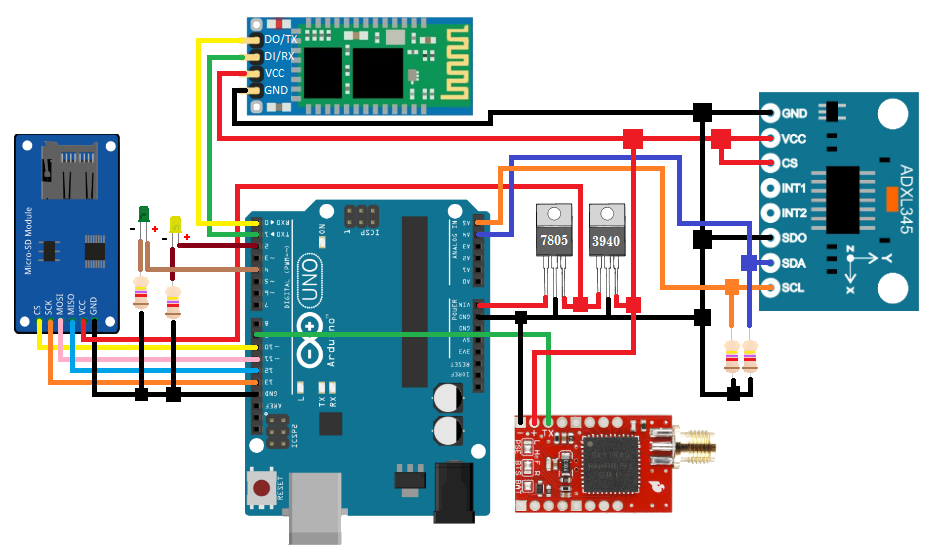
\includegraphics[width=15cm]{esquema}
	\caption{Esquemático do sistema}
	\label{fig:esquematico_do_sistema}
\end{figure}

\begin{figure}[htbp]
	\centering
	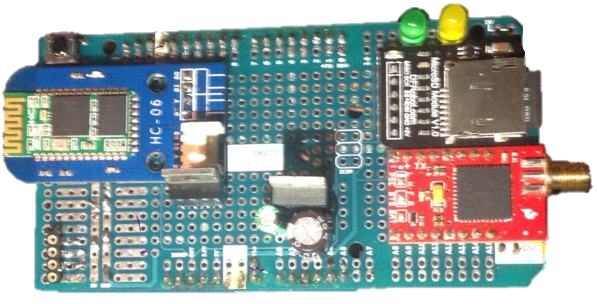
\includegraphics[width=10cm]{montagem}
	\caption{Montagem real do sistema}
	\label{fig:montagem_real_do_sistema}
\end{figure}

\begin{figure}[htbp]
	\centering
	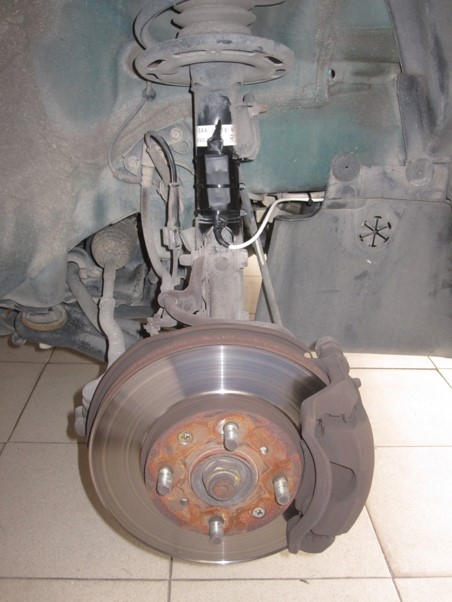
\includegraphics[height=10cm]{carro}
	\caption{Instalação do sensor no veículo de testes}
	\label{fig:carro}
\end{figure}

\section{Validação de resultados}
\label{sec:validacao}

De modo a fazer uma validação do sistema e dos seus resultados, o sistema foi parcialmente montado num veículo de testes, mantendo o acelerómetro no seu interior para que fossem inseridas irregularidades manualmente, apesar do bom estado do pavimento.
Este teste serviu para confirmar o bom funcionamento de todo o sistema, ou seja, o acelerómetro e o GPS, a comunicação Bluetooth e 3G e também a base de dados e web site para consulta de dados inseridos.
Na figura \ref{fig:validacao} é possível consultar o percurso deste teste.

\begin{figure}[htbp]
	\centering
	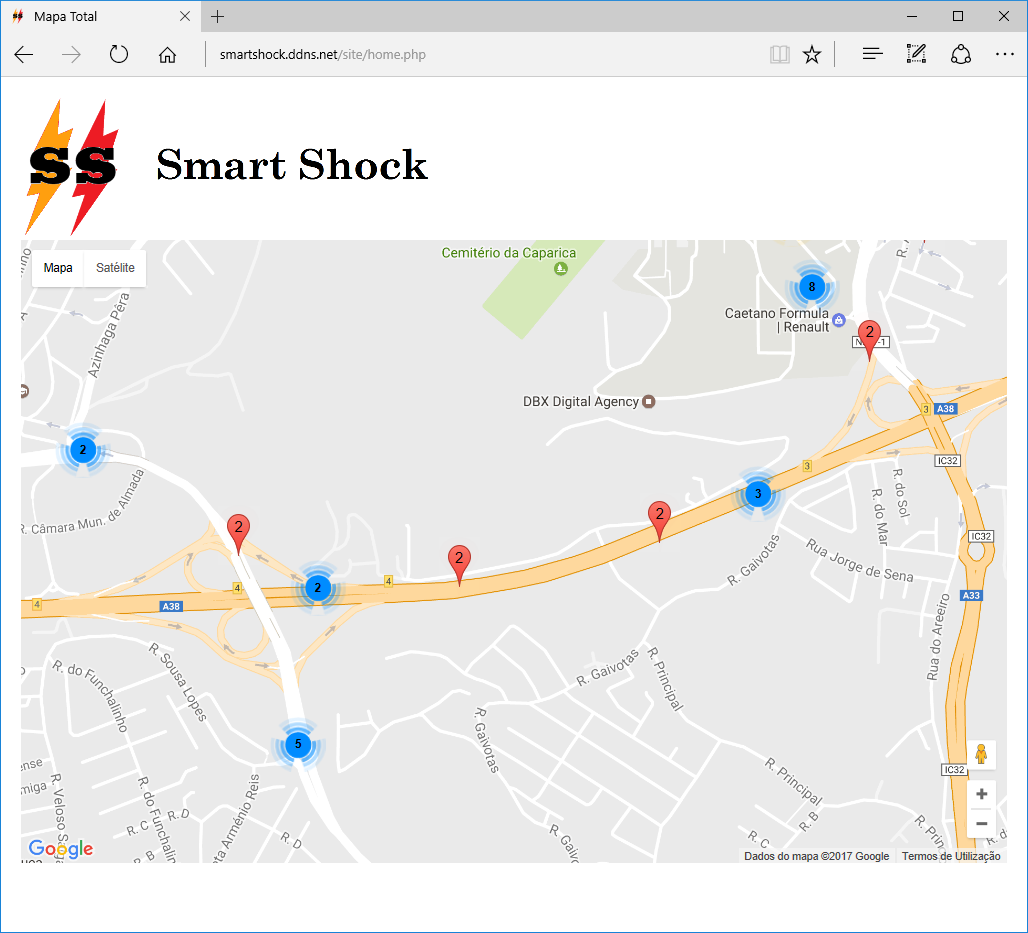
\includegraphics[height=10cm]{Validacao}
	\caption{Percurso de validação de resultados}
	\label{fig:validacao}
\end{figure}

Após concluir que todo o sistema estava a funcionar corretamente, o acelerómetro foi montado no automóvel e foram adquiridos dados ao longo de vários dias para que a base de dados ficasse mais completa.
Apesar de não existir uma análise destes dados, o sistema mostrou funcionar em perfeitas condições, fazendo deteções regularmente sempre que o veículo passava por alguma irregularidade.
Na análise do mapa, é possível verificar que algumas deteções se encontram fora das estradas, algo impossível de acontecer no cenário real.
Ainda assim, o afastamento nunca é superior a 5 metros, a escala menor do mapa, sendo esse um valor aceitável neste tipo de sistemas pois à escala humana facilmente se identificam todas irregularidades que estejam a 5 metros de distância de um determinado ponto.

\section{Resultados obtidos}
\label{sec:resultados}

Tal como esperado, o sistema apresentou resultados positivos quanto à deteção de irregularidades no asfalto.
O acelerómetro é um sistema fiável no que diz respeito a este tipo de deteção e a sua calibração é praticamente inexistente tendo em conta a montagem proposta, tornando este sistema bastante fácil de usar e apelativo.
O recetor GPS também apresentou resultados bastante fiáveis e consistentes ao longo de todos os testes feitos, mesmo aqueles em que o sistema não se encontrava totalmente montado.

A aplicação também mostrou ser útil como ponto intermédio de comunicação.
O seu desenho simples torna muito intuitiva a utilização sendo apenas necessário selecionar o dispositivo com que se deseja comunicar.
Para a comunicação à base de dados é apenas necessário que exista ligação à Internet, não existindo qualquer diferença quanto ao modo de ligação, seja ele Wi-Fi ou 3G.
É ainda possível determinar que, através do App Inventor, a construção da aplicação foi bastante rápida e intuitiva, reduzindo significativamente o tempo de desenvolvimento e de teste da mesma.

Por fim, a base de dados fez um armazenamento de dados sem qualquer tipo de problemas.
A configuração da mesma foi bastante fácil e a sua consulta em SQL é totalmente adequada aos requisitos deste projeto.
A construção das páginas \emph{web} à volta dos dados da aplicação serviu para que a consulta de dados fosse mais prática.
A utilização do Google Maps e das suas funcionalidades possibilitou a utilização de um mapa interativo para que fosse mais direta a identificação da localização das irregularidades detetadas.